%\chapter{Introduction to Linear Programming}
\chapter{Geometry and Duality for Linear Programming}
\section{The polyhedral geometry}
The constraint of a LP forms a polyhedron. One example for a LP with tenary variables is shown in the Fig~(\ref{fig:2:1})
\begin{figure}
\centering
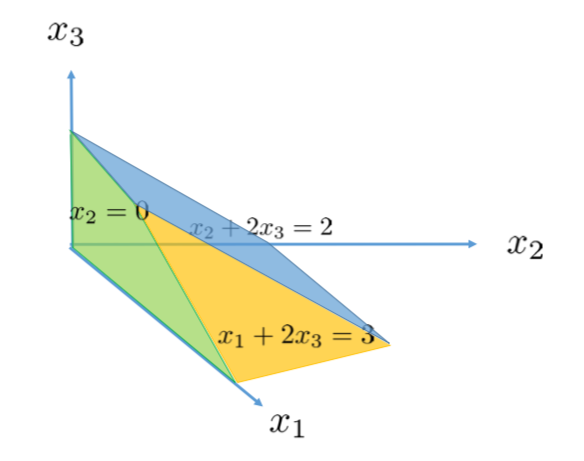
\includegraphics[width=0.5\textwidth]{Second_lecture/p_1}
\caption{Illustration for polyhedral geometry}
\label{fig:2:1}
\end{figure}

Let's introduce some terminologies formally:
\begin{definition}
\begin{itemize}
\item
\emph{Hyperplane} is the set $\{\bm x\mid \bm a\trans\bm x=\bm b\}$
\item
\emph{Half-space} is the set $\{\bm x\mid\bm a\trans\bm x\le\bm b\}$
\item
The \emph{polyhedron} $P$ is the intersection of \emph{finite} number of half-spaces:
\[
P=\left\{
\bm x\middle|
\bm a_i\trans \bm x\le \bm b_i,
\ i=1,\dots,m
\right\}
\]
\item
The \emph{dimension of a polyhedron} is defined as the \emph{lowest} dimension \emph{affine space} containing $P$
\item
The \emph{face} of a polyhedron is defined as
\[
\{\bm x\mid \bm a\trans\bm x=\bm b\}\cap P,
\]
where $P\subseteq\{\bm x\mid \bm a\trans\bm x\le\bm b\}$.
\item
Note that the face of a polyhedron is also a polyhedron. Therefore we define \emph{facet} is the face of $P$ that is one dimensional lower than that of $P$; the \emph{vertex} of $P$ is the face of $P$ that has dimension $0$.
\end{itemize}
\end{definition}
\begin{remark}
In space $\mathbb{R}^n$, normally $n$ hyperplanes intersect at one point
\item
If $P$ is full dimensional (i.e., with diemension $n$), then a vertex of $P$ is an intersection of $n$ facets.
\item
However, sometimes there is a case that more than $n$ hyperplanes intersect at one point, say a vertex, which creates \emph{degeneracy} (show in Fig~(\ref{fig:2:2})).
In such case, adding regularization, i.e., perturbation dimishes over-determination.
\end{remark}
\begin{figure}
\centering
\begin{minipage}[t]{0.48\textwidth}
\centering
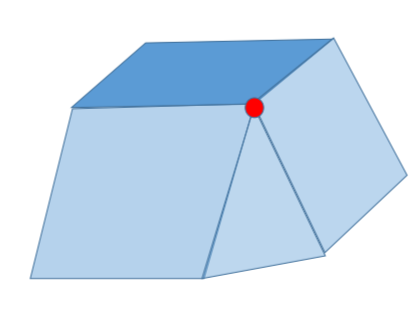
\includegraphics[width=1\textwidth]{Second_lecture/p_2}
\caption{Over-determination results in Degeneracy}
\label{fig:2:2}
\end{minipage}
\begin{minipage}[t]{0.48\textwidth}
\centering
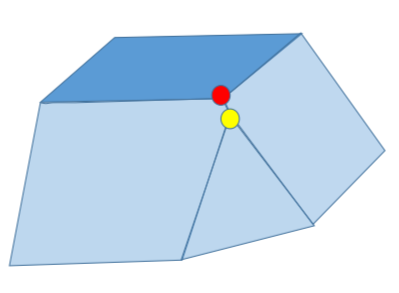
\includegraphics[width=1\textwidth]{Second_lecture/p_3}
\caption{Perturbation diminishes over-determination}
\label{fig:2:3}
\end{minipage}
\end{figure}

\begin{definition}
Given a full dimensional $P$, we say two distinct vertices of $P$ are \emph{adjacent} if they are in the same $n-1$ hyperplane.
\end{definition}
\begin{remark}
Every update for simplex pivots move from a vertice to one of its adjacent position.
\end{remark}
\begin{figure}
\centering
\begin{minipage}[t]{0.48\textwidth}
\centering
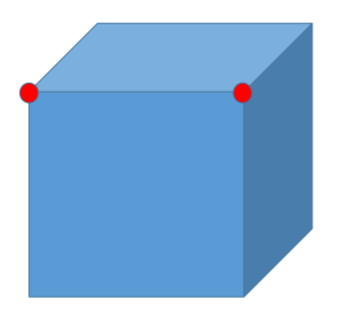
\includegraphics[width=1\textwidth]{Second_lecture/p_4}
\caption{Illustration for \emph{adjacent} vertices}
\label{fig:2:2}
\end{minipage}
\begin{minipage}[t]{0.48\textwidth}
\centering
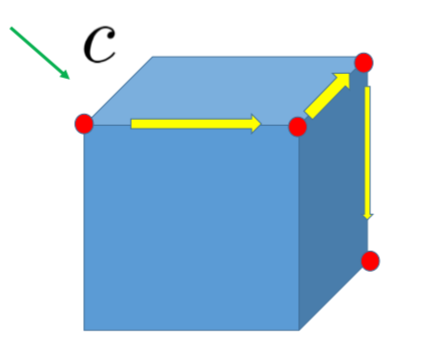
\includegraphics[width=1\textwidth]{Second_lecture/p_5}
\caption{Path for simplex pivots}
\label{fig:2:3}
\end{minipage}
\end{figure}

\begin{definition}
A \emph{polyhedral cone} is defined as an intersection of a finite number of half-spaces, i.e., 
$K=\{\bm x\in\mathbb{R}^n\mid \bm A\bm x\ge\bm0\}$, where $\bm A\in \mathbb{R}^{m\times n}$. In geometry shown in Fig~(\ref{fig:2:4}), a polyhedral cone is a cone where its boundaries are polyhedral
\end{definition}
\begin{figure}
\centering
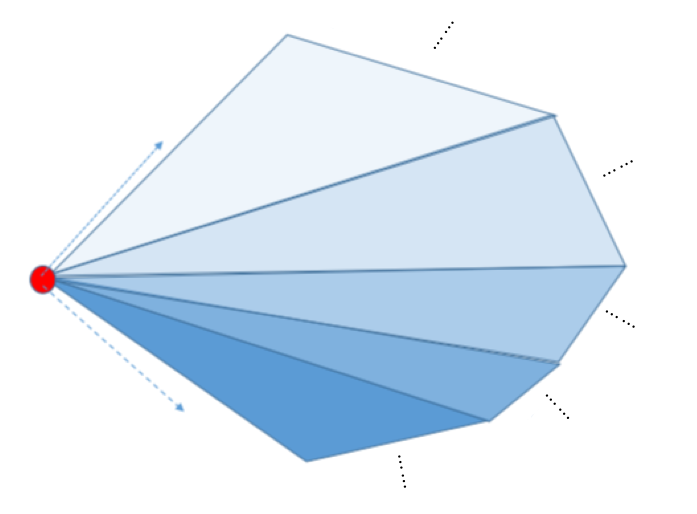
\includegraphics[width=0.48\textwidth]{Second_lecture/p_6}
\caption{Illustration for a polyhedral cone}
\label{fig:2:4}
\end{figure}

\begin{definition}
Given a set of points $S$, we can define its convex hull as
\[
\text{conv hull}(S):=
\left\{
\sum_{i=1}^m\lambda_i \bm y_i\middle|\ 
\forall \bm y_i\in S,
\lambda_i\ge0,
\sum_{i=1}^m\lambda_i=1
\right\}
\]
In other words, a convex hull of $S$ is a set, in which each point is a convex combination of points in $S$.
\end{definition}
\begin{figure}
\centering
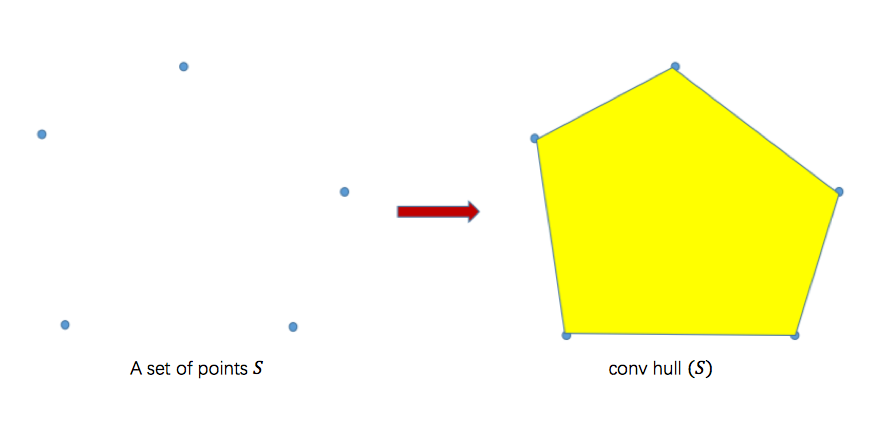
\includegraphics[width=0.9\textwidth]{Second_lecture/p_7}
\caption{Illustration for a convex hull}
\label{fig:2:5}
\end{figure}

\section{Fundamental Theorems for Linear Programming}
\begin{theorem}[Caratheodory’s Theorem]
Let $P\subseteq \mathbb{R}^n$ be a set of points.
For each $\bm x\in\text{conv}(P)$, there exists a set $P'\subseteq P$ of cardinality at most $n+1$,
such that $\bm x\in\text{conv}(P')$.
\end{theorem}

\begin{definition}
The point $\bm x$ in a convex set $S$ is an \emph{extremal point} if
\begin{enumerate}
\item
$x\in S$
\item
$x$ is a convex combination of $y,z\in S$ implies $y=z=x$.
\end{enumerate}
\end{definition}

Sometimes it is difficult to define the extremal point, if the convex set covers infinite area. Therefore, we define the points in the boundary of vertices instead:
\begin{definition}
A ray $d$ in a convex cone $\mathcal{K}$ is an \emph{extremal ray} if
\begin{enumerate}
\item
$d\in\mathcal{K}$
\item
If $d$ can be written as non-negative summation of two rays $\xi_1,\xi_2\in\mathcal{K}$, then $d=\xi_1=\xi_2$
\end{enumerate}
\end{definition}

\begin{definition}
\begin{enumerate}
\item
A \emph{polytope} is a convex hull of a \emph{finite} number of points
\item
A \emph{polytope} is also a \emph{polyhedron}
\item
In general, a polyhedron can be written as
\[
\left\{
\sum_{i=1}^m\lambda_ip_i
+
\sum_{j=1}^{\ell}\mu_jd_j
\middle|\
\lambda_i\ge0,
\sum_{i=1}^m\lambda_i=1,
\mu_j\ge0
\right\}
\]
In other words, 
\[
H=P+C,
\]
where $H,P,C$ denote collections of polyhedrons,polytopes,polyhedral cones, respectively.
\end{enumerate}
\end{definition}

\begin{definition}
If $\mathcal{K}$ is a convex cone, then its \emph{dual cone} is defined as
\[
\mathcal{K}^*=\{\bm s\mid\inp{\bm s}{\bm x}\ge0,\ \forall \bm x\in\mathcal{K}\}.
\]
\end{definition}

The Fig~(\ref{fig:2:6}) represents one illustration for convex cone and its dual cone, but note that the dual cone may not necessarily larger than the convex cone itself. (Counter-example: Lorentz cone)
\begin{figure}
\centering
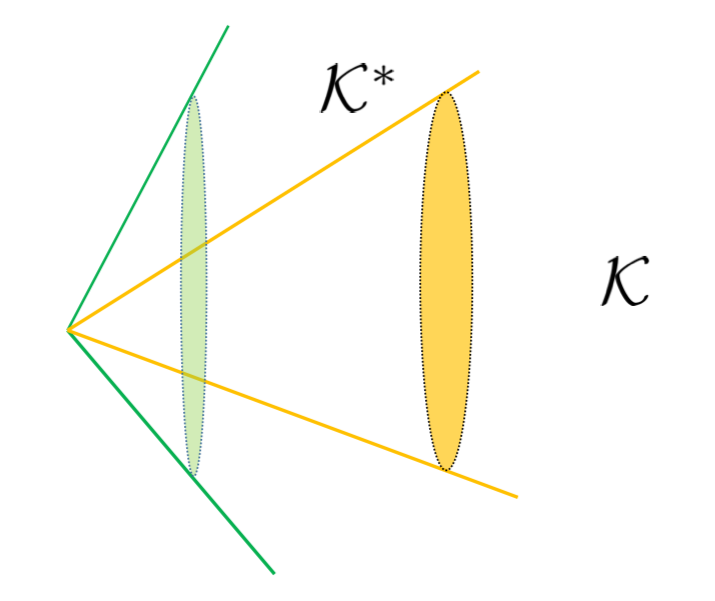
\includegraphics[width=0.48\textwidth]{Second_lecture/p_8}
\caption{Illustration for a convex cone and its dual cone}
\label{fig:2:6}
\end{figure}

A polyhedral cone can be represented in two ways:
\[
\begin{array}{lll}
\{\bm A\bm x\mid\bm x\ge0\}
&
\mbox{and}
&
\{\bm x\mid \bm B\trans\bm x\ge0\}
\end{array}
\]

Here we consider two cones $\{\bm A\bm x\mid \bm x\ge0\}$ and $\{\bm y\mid\bm A\trans\bm y\ge0\}$:
\begin{theorem}
Two cones $\mathcal{K}_1=\{\bm A\bm x\mid \bm x\ge0\}$ and $\mathcal{K}_2=\{\bm y\mid\bm A\trans\bm y\ge0\}$ are actually \emph{duality pairs}.
\end{theorem}
\begin{proof}
It's obvious that $\{\bm A\bm x\mid\bm x\ge0\}\subseteq\{\bm y\mid\bm A\trans\bm y\ge0\}^*$.

Given that $\bm b\notin \{\bm A\bm x\mid\bm x\ge0\}$, there exists $\bm y$ such that $\bm A\trans\bm y\ge0$ and $\inp{b}{y}<0$ (by Farkas Lemma), i.e., $\bm b$ cannot be in $\{\bm y\mid\bm A\trans\bm y\ge0\}^*$.
\end{proof}

\begin{theorem}[Farkas Lemma]\label{The:2:3}
If $\bm b\notin\{\bm A\bm x\mid\bm x\ge0\}$, then there exists $\bm y$ such that $\bm A\trans\bm y\ge0$ and $\inp{\bm b}{\bm y}<0$.
\end{theorem}
An equivalent form of Farkas Lemma is as follows (known as the \emph{theorem of alternatives}):
\begin{quotation}
Either $\bm A\bm x=\bm b,\bm x\ge0$ has a solution, or $\bm A\trans\bm y\ge0,\inp{\bm b}{\bm y}=-1$ has a solution, but not neither, nor both.
\end{quotation}

\begin{proof}
Consider the primal LP
\[
(P)\qquad
\begin{array}{ll}
\max&-\bm s\\
\mbox{such that}&\bm A\bm x+\bm s\bm b=\bm b,\\
&\bm x\ge0,\bm s\ge0
\end{array}
\]
The dual LP is
\[
(D)\qquad
\begin{array}{ll}
\min&\inp{\bm b}{\bm y}\\
\mbox{such that}&\bm A\trans\bm y\ge0\\
&\inp{\bm b}{\bm y}\ge-1 
\end{array}
\]
Since the primal problem is feasible and bounded, and so an optimal solution exists.
By strong duality theorem, $\{\bm x\mid\bm A\bm x=\bm b,\bm x\ge0\}=\emptyset$ iff the (D) admits negative optimal value. 
\end{proof}

\begin{remark}
The Farkas Lemma essentially claims that given a polyhedron $\mathcal{K}_1=\{\bm x\mid\bm A\bm x=\bm b,\bm x\ge0\}$ and a point $\bm y$ outside $\mathcal{K}_1$, we can always find an affine that separates $\mathcal{K}_1$ and $\bm y$ (see Fig~(\ref{fig:2:9}))
\begin{figure}
\centering
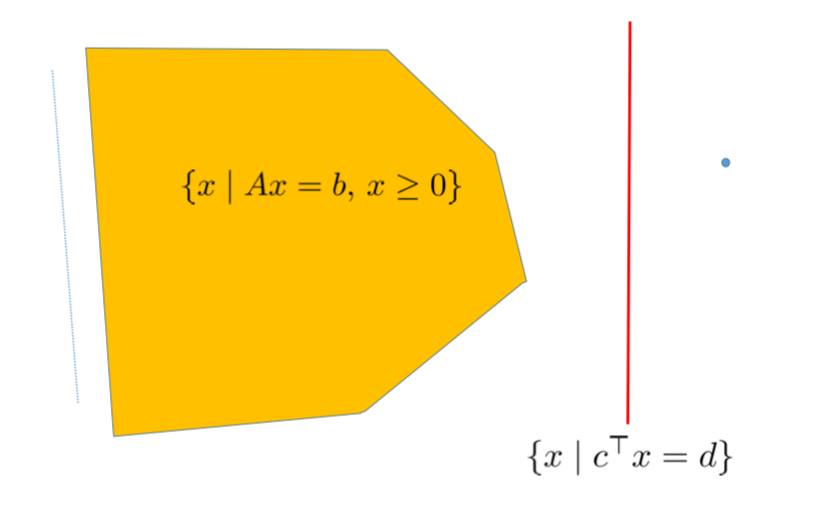
\includegraphics[width=0.9\textwidth]{Second_lecture/p_9}
\caption{Illustration for the separation of $\mathcal{K}_1$ and $\bm y$}
\label{fig:2:9}
\end{figure}

Actually, we can generalize this separation into general polyhedron.
\end{remark}
\begin{theorem}[Separation Theorem]
Let $H\subseteq\mathbb{R}^n$ be a general \emph{polyhedron}. Suppose that $\mathbb{R}^n\ni \bm p\notin H$, then there exists an affine $f(\bm x)=\bm c\trans\bm x+\bm d$ satisfying
\[
\begin{array}{ll}
f(\bm p)<0,&
f(\bm x)=\bm c\trans\bm x+\bm d>0,\forall\bm x\in H
\end{array}
\]
\end{theorem}

\begin{proof}
Consider a general polyhedron $H$ with vertices $\{\bm p_i\mid i=1,\dots,m\}$ and extreme rays $\{\bm d_j\mid j=1,\dots,\ell\}$. Since $\bm p\notin H$, the system (\ref{Eq:2:1}) does not have a solution:
\begin{equation}\label{Eq:2:1}
\begin{aligned}
\bm p&=\sum_{i=1}^m\lambda_i\bm p_i+\sum_{j=1}^\ell\mu_j\bm d_j\\
1&=\sum_{i=1}^m\lambda_i\\
0&\le\lambda_i,\quad i=1,\dots,m\\
0&\le\mu_j,\quad j=1,\dots,\ell
\end{aligned}
\end{equation}

By Farkas Lemma, there exists $\bm y\in\mathbb{R}^n$ and $\bm s\in\mathbb{R}$ such that
\begin{align*}
\bm s+\bm p_i\trans\bm y&\ge0,\quad i=1,\dots,m\\
\bm d_j\trans\bm y&\ge0,\quad j=1,\dots,\ell\\
\bm s+\bm p\trans\bm y&<0
\end{align*}

\end{proof}

\begin{remark}
It's also easy to derive the Farkas Lemma from the Separation Theorem:

Suppose $\bm b\notin \{\bm A\bm x\mid\bm x\ge0\}$, then there is a separating hyperplane $\bm c\trans\bm z= d$, such that
\[
\begin{array}{ll}
\bm c\trans\bm b< d,
&
\bm c\trans\bm z> d,\forall \bm z=\bm A\bm x,\text{ with }\bm x\ge0
\end{array}
\]
which implies that $\bm A\trans\bm c\ge0,d<0,\bm c\trans\bm b<d$.
\end{remark}

There are different ways to show the same result. Our previous proof of Theorem~(\ref{The:2:3}) is based on the \emph{finiteness of the simplex method}, i.e., the duality of LP. Terence Tao applied a different and more direct method to show the Farkas Lemma, let's study it in detail.

First we aim to show the Farkas Lemma in the dual way:
\begin{theorem}[Rephrased Form of Farkas Lemma]
Let $P_i(x)=\sum_{j=1}^np_{ij}x_j - r_i, i=1,\dots,m$.
If the system $P_i(x)\ge0$ for $i=1,\dots,m$ does not have a solution, 
then there exists $y_i\ge0$ such that
$
\sum_{i=1}^my_iP_i(x)=-1.
$
\end{theorem}

\begin{proof}
We can show this result by induction on $n$:
\begin{itemize}
\item
When $n=1$, we can scale $P_i(x)\ge0$ possibly into three cases:
\[
\begin{array}{lll}
x_1-a_i\ge0,\ i\in I_+;
&
-x_1+b_j\ge0,\ j\in I_-;
&
c_k\ge0, \ k\in I_0
\end{array}
\]

If there exists $k\in I_0$ with $c_k<0$, we let $y_k = -1/c_k$ and $y_\ell = 0,\forall \ell\ne k$; otherwise there exists $i\in I_+$ and $j\in I_-$ with $a_i>b_j$, we let $y_i=y_j=1/(a_i-b_j)$ and $y_\ell =0,\forall \ell\ne i,j$. Therefore, we obtain $\sum_{i=1}^my_iP_i(x)=-1$.
\item
Now suppose that this theorem is shown for dimension no more than $n$. Consider the case where we have $n+1$ variables: $\bar{\bm x} = (\bm x,x_{n+1})$, $\bm x\in\mathbb{R}^n$.
We can scale the original inequalities over $P_i(\bar{\bm x})$ according to the coefficients of $x_{n+1}$ to obtain the following equivalent system of inequalities:
\begin{equation}
\left\{
\begin{aligned}
P_i(\bar{\bm x}):&=x_{n+1} - Q_i(\bm x)\ge0,\quad i\in I_+\\
P_j(\bar{\bm x}):&=-x_{n+1} - Q_j(\bm x)\ge0,\quad j\in I_-\\
P_k(\bar{\bm x}):&=Q_k(\bm x)\ge0,\quad k\in I_0
\end{aligned}
\right.
\end{equation}

Note that the system
\begin{equation}\label{Eq:2:3}
\left\{
\begin{aligned}
-Q_i(x)+Q_j(x)&\ge0,\quad i\in I_+,j\in I_-\\
Q_k(x)&\ge0,\quad k\in I_0
\end{aligned}
\right.
\end{equation}
has a solution implies that the original system would have a solution too. 
Due to the hypothesis of the lemma, (\ref{Eq:2:3}) does not have a solution.

By the induction hypothesis, there exists $y_{ij},y_k\ge0$ such that
\[
\sum_{i\in I_+, j\in I_-}y_{ij}(-Q_i(x) + Q_j(x)) + \sum_{k\in I_-}y_kQ_k(x)=-1
\]

Therefore, we imply
\begin{align*}
\sum_{i\in I_+}\left(\sum_{j\in I_-}y_{ij}\right)(x_{n+1} - Q_i(x))&
+
\sum_{j\in I_-}\left(\sum_{i\in I_+}y_{ij}\right)(-x_{n+1} + Q_j(x))\\
&+
\sum_{k\in I_0}y_kQ_k(x)=-1
\end{align*}

\end{itemize}
The Farkas Lemma is shown by this induction argument.
\end{proof}

Then we are ready to show the following form of separation theorem:

\begin{theorem}[Repharsed Form of Separation Theorem]
If polytopes $P_1,P_2$ do not intersect, then there is an affine $f(\bm x)=\inp{\bm y}{\bm x}+y_0$ such that 
\[
\begin{array}{ll}
f(\bm x)\ge1,\ \forall \bm x\in P_1
&
f(\bm x)\le 1,\ \forall \bm x \in P_2
\end{array}
\]
\end{theorem}
\begin{proof}
Suppose the extreme points of $P_1,P_2$ are $\{\bm p_1,\dots,\bm p_s\}$ and $\{\bm q_1,\dots,\bm q_t\}$, respectively. Therefore, it suffices to show that
\begin{equation}\label{Eq:2:4}
\begin{array}{ll}
\inp{\bm y}{\bm p_i}+y_0\ge1, \ i=1,\dots,s;
&
\inp{\bm y}{\bm q_j}+y_0\le-1,\ j=1,\dots,t
\end{array}
\end{equation}

Suppose on the contrary that (\ref{Eq:2:4}) does not have a solution $(\bm y,\bm y_0)$.
Then the Farkas Lemma asserts that there exists $u_i\ge0, i=1,\dots,s$ and $v_j\ge0, j=1,\dots,t$ such that
\[
\sum_{i=1}^su_i(\inp{\bm y}{\bm p_i} + y_0 - 1)
+
\sum_{j=1}^tv_j(-\inp{\bm y}{\bm q_j} - y_0 - 1)
=-1
\]
which implies
\begin{align*}
\sum_{i=1}^su_i\bm p_i - \sum_{j=1}^tv_j\bm q_j&=0\\
\sum_{i=1}^su_i - \sum_{j=1}^tv_j &= 0\\
\sum_{i=1}^su_i + \sum_{j=1}^tv_j&=1
\end{align*}

Therefore, $\sum_{i=1}^su_i = \sum_{j=1}^tv_j = 1/2$, and thus
\[
P_1\ni
2\sum_{i=1}^su_i\bm p_i
=
2\sum_{j=1}^tv_j\bm q_j
\in P_2
\]
which contradicts to the assumption that $P_1\cap P_2=\emptyset$.
\end{proof}
The same argument applies if \emph{polytopes} is replaced by \emph{polyhedron}.

\section{More Theorems of Alternatives: the case for polyhedrons}
Some more refined forms of the theorems of alternatives exist. Here we list some examples.

\paragraph{Notations}
Let $\bm x,\bm y$ be two vectors, we denote $\bm x\gvertneqq\bm y$ to be ``$\bm x\ge\bm y$ and $\bm x\ne\bm y$'', and similarly for $\bm x\lvertneqq\bm y$.

\begin{theorem}[Gordan]\label{The:2:7}
Either $\bm A\bm x>0$ has a solution, or $\bm A\trans\bm y=0,\bm y\gvertneqq0$ has a solution.
\end{theorem}

\begin{theorem}[Stiemke]
Either $\bm A\bm x\gvertneqq0$ has a solution, or $\bm A\trans\bm y=0,\bm y>0$ has a solution.
\end{theorem}

\begin{theorem}[Gale]
Assuming $\bm A\bm x\le\bm b$ is feasible, then either $\bm A\bm x\lvertneqq\bm b$ has a solution, or $\bm A\trans\bm y=0,\bm b\trans\bm y=0,\bm y>0$ has a solution.
\end{theorem}

\begin{theorem}[Tucker]
Suppose that $\bm A\ne\bm0$. Either 
$\bm A\bm x\gvertneqq0,\bm B\bm x\ge0,\bm C\bm x=0$ has a solution,
or $\bm A\trans\bm u+\bm B\trans\bm v+\bm C\trans\bm w=0,\bm u>0,\bm v\ge0$
has a solution.
\end{theorem}

\begin{theorem}[Motzkin]
Suppose that $\bm A\ne\bm0$. Either 
\[
\bm{Ax}>0,\bm B\bm x\ge0,\bm C\bm x=0
\]
has a solution, or
\[
\bm A\trans\bm u+\bm B\trans\bm v+\bm C\trans\bm w=0,
\bm u\gvertneqq0,
\bm v\ge0
\]
has a solution.
\end{theorem}





















